\section{Evaluation}
\label{sec:eval}

In this section we present an empirical evaluation of \quark on two
case studies. First is a collaborative document editing
application -- a common usecase addressed by several CRDT
proposals~\cite{rga, treedoc, crdts}. Second is a replicated key-value
store implemented using a mergeable Red-Black tree data structure.

\subsection{Collaborative Editing}

\quark's MRDT approach obviates the need to build a dedicated
replicated data type for collaboratively-edited documents; an ordinary
document format extended with a merge operation would suffice. While
many data structures exist to represent text documents (e.g.,
ropes~\cite{boehm95}), we decided to adopt the simplest representation
of a document as a list of characters. 
\begin{center}
\begin{ocaml}
        type doc = char list
\end{ocaml}
\end{center}
While being simple, the advantage of this presentation is that we can
simply reuse the three-way \C{List.merge} function of the list data
type to merge documents. \C{List.merge} is a simple implementation of
list merge algorithm (in ~60 lines of OCaml) inspired by the GNU
\C{diff3} algorithm~\cite{gnudiff}. We thus adopt a straightforward
approach to building a collaborative document editor with the
intention to keep the development effort low enough to be easily
replicated. The convergence guarantee of \quark ensures that the
simplicity of our implementation doesn't come at the expense of
correctness. The aim of the experimental evaluation is to quantify the
impact of \quark on the performance.

Our experiment setup consists of multiple collaborators simultaneously
editing a 10000+ line document obtained from the Canterbury
Corpus~\cite{canterbury}. Each user holds a replica of the document
and is assumed to be editing the document at the speed of 240
characters per minute or 1 character every 0.25s. At 6 characters per
word, this amounts to 40 words per minute, which is the average typing
speed of humans. Each edit is immediately persisted to the disk by
creating a new version in the backing store. Thus there are at least
as many versions of the document as there are edits. Such extensive
versioning may be considered excessive in practice and could be
disabled. 

\noindent\paragraph{Latency} To measure the impact of \quark runtime on user
writes, we measure the latency of the \C{write} operation, which
includes the time spent merging the user version with the current
version, and persisting the resultant version to the store. We conduct
the experiments on a three-node cluster of \C{i3.large} machines
located in Amazon \C{us-west2} data center. Each user connects to one
of the machines, forks a new branch, and performs 1000 edits in
succession, saving the document after each edit. We progressively
increase the number of concurrent users editing the document from 3 to
60 and measure the impact of the increased concurrency on write
latency.  Fig.~\ref{fig:latency} shows the 10th, 50th (median), and
90th percentile latency values. The median and 10th percentile
latencies remain more-or-less constant with a slight increase between
3 and 60 concurrent users. This is expected considering that \quark
does not constrain the execution of user operations. The slight
increase, we confirmed, is due to the increased latency of concurrent
database writes. The 90th percentile latencies, however, show an
initial increase before adopting a pattern similar to median
latencies. We attribute this behavior to an idiosyncrasy of our
multi-threading implementation, which is more likely to affect
measurements at the extreme. In particular, we use OCaml v4.12
extended with Lightweight Threads (LWT) library, which offers
concurrency but not parallelism.  At lower number of replicas, the
merge thread's lock requests succeed more often, resulting in the
process spending more time merging than editing. We expect this
pattern to smoothen out in OCaml v5.0, which introduces true
multi-core parallelism. Notwithstanding this idiosyncrasy, the maximum
value of 90th percentile latency measured (32ms) remains well below
the the time between consecutive edits (0.25s), making it hard to
perceive by a human user. 

\begin{figure}[ht]
  \centering
    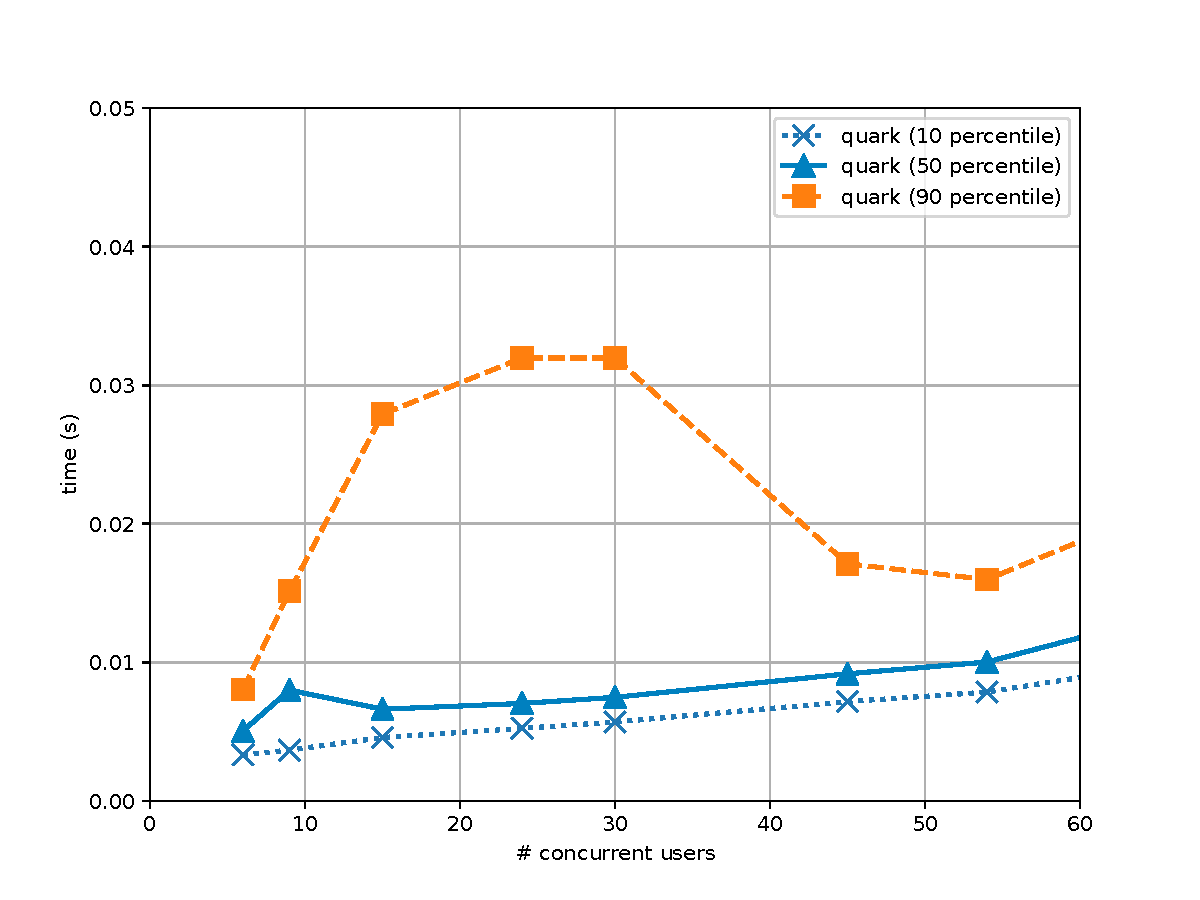
\includegraphics[scale=0.4]{Figures/monkey_latency}
\caption{Latency of writes to a shared document under \quark. }
\label{fig:latency}
\vspace*{-0.1in}
\end{figure}

For comparison against a baseline, we have implemented an ``SC''
approach which achieves convergence by synchronizing each operation,
i.e., executing it under strong consistency (SC). The SC
implementation shares most of its code with \quark with the only
change being that it wraps commits instead of merges inside a lock.
As with \quark, we measured the write latency of the SC implementation
while increasing the number of concurrent users ($n$).  The median SC
write latency increases super-linearly from 10ms for $n=3$ to 63s
(i.e., >1m) for $n=60$, which is considerably more than the inter-edit
latency of 0.25s.


\noindent\paragraph{Staleness} Our implementation of \quark relies on
Scylla to replicate the contents of each branch across all the
replicas as fast as the network allows. However, for a user $A$ to see
the changes made by the other user $B$, the changes have to be
reflected in $A$'s local version, which can only happen through a
merge operation. Since \quark synchronizes merge operations globally,
it induces additional delay before $A$ can see $B$'s changes. We call
this additional delay \emph{staleness} as with the progression of
time, $B$'s version known to $A$ becomes increasingly stale. At the
system-level, an increase in staleness effectively delays the
convergence (but doesn't preempt it, as proved by
Theorem~\ref{thm:progress}). 

\begin{figure}[ht]
  \centering
    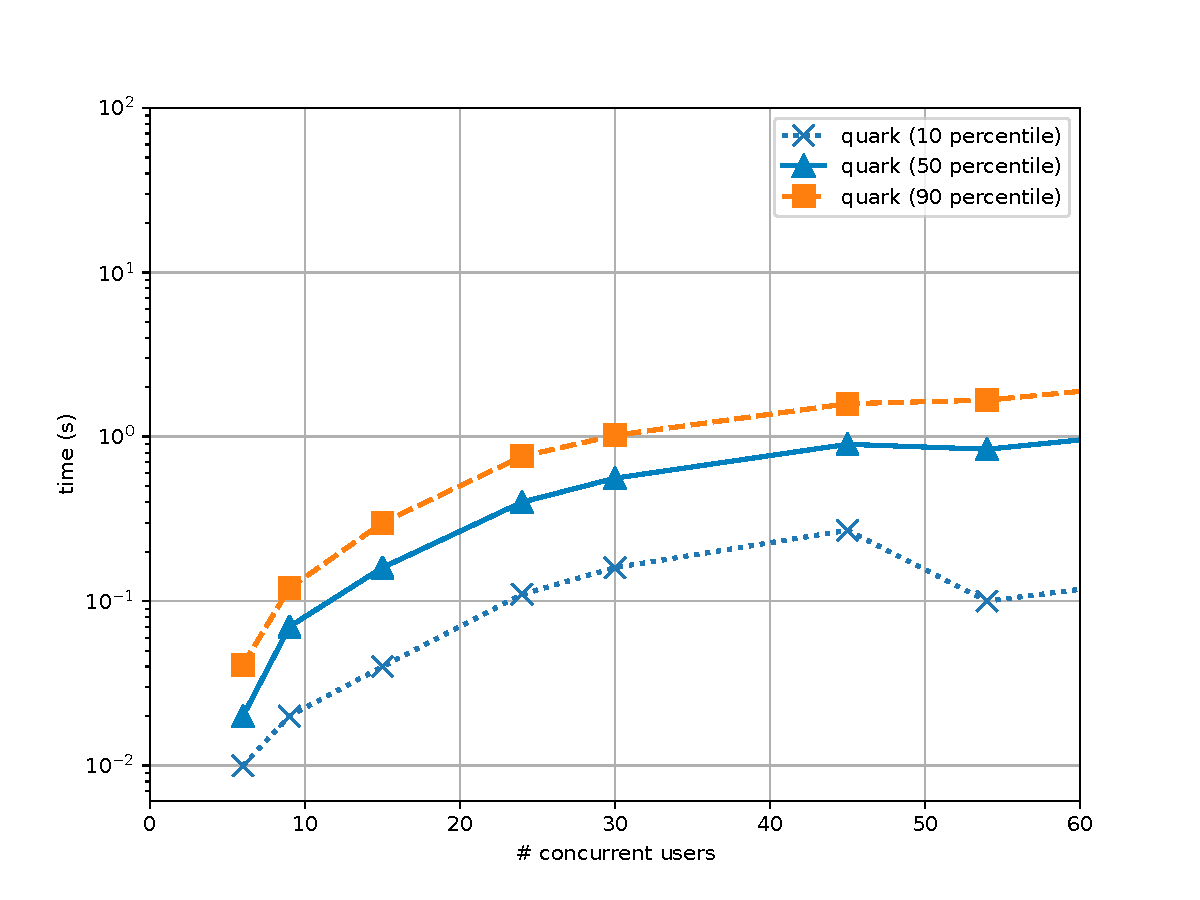
\includegraphics[scale=0.4]{Figures/monkey_staleness}
\caption{Staleness increases as the number of concurrent editors
  increase.}
\label{fig:monkey-staleness}
\vspace*{-0.2in}
\end{figure}

To understand the effect of \quark on
staleness, we quantify and measure it along with latency in the
experiment setup described above. Staleness is defined as the time
taken for a version committed on one replica to be merged into a
concurrent version on a remote replica. To measure staleness, we
annotate every version $v$ with the timestamp $t$ of the wall clock
time of its creation. When $v$ is is merged into a remote branch $b$
at a later time $t'$, the difference $t' - t$ denotes the staleness of
$v$ w.r.t the new version on $b$. One such staleness measurement is
recorded for every merge that ever happens during the experiment. We
compute 10th, 50th, and 90th percentiles of staleness values thus
obtained. Fig.~\ref{fig:monkey-staleness} shows the results. As
evident, staleness increases steadily with the increasing number of
concurrent replicas, which is expected considering that merges are
synchronized, and increasing the number of replicas reduces the number
of opportunities for a replica to merge. The increase is roughly
linear in the number of replicas as our implementation passes the lock
around in a round-robin fashion. Despite the steady increase, the 90th
percentile staleness values remain low -- less than 1s with the
number of replicas under 30, and less than 2s for number of replicas
under 60. While further optimizations might reduce staleness, a
non-trivial staleness overhead is inevitable in \quark due to our use
of synchronized merges to guarantee convergence. 

% Our approach thus
% introduces staleness as novel tradeoff against convergence. While
% trading off staleness may not be an optimal choice for every
% application, it is arguably a less disruptive choice if an application
% has to choose between latency and staleness.
% Sec.~\ref{sec:motivation}\footnote{
%   Git admits anamolous version history graphs where two branches can
%   have the same set of commits and yet differ in their final version.
%   Supplementary material describes two such cases we observed on
%   Github.}. 

\subsection{Key-Value Store}

Our second case study involves a mergeable key-value store, which,
unlike a text editor, is expected to work in the background supporting
applications such as e-Commerce. The store is mergeable in the sense
that it can merge conflicting values assigned to equal keys using
value-specific merge functions. For instance, an e-Commerce
application might store shopping carts as values, in which case the
merge function on shopping carts is used to merge concurrent
conflicting updates to a user's shopping cart. The key-value store is
implemented using a Red-Black tree MRDT~\cite{mrdt}, which is a
standard Red-Black tree implementation extended with a merge function.
The merge function implements set merge semantics
(Sec.~\ref{sec:motivation}) for concurrent insertions and deletions of
keys, and defers to the value merge function for concurrent updates
against a key. Concretely, \C{RBTree} is an OCaml functor
parameterized on the \C{Key} and \C{Value} modules, where the latter
is required to provide a \C{merge} function. We use integer keys and
mergeable counter values in our experiments.

% \begin{figure}[ht]
%   \centering
%     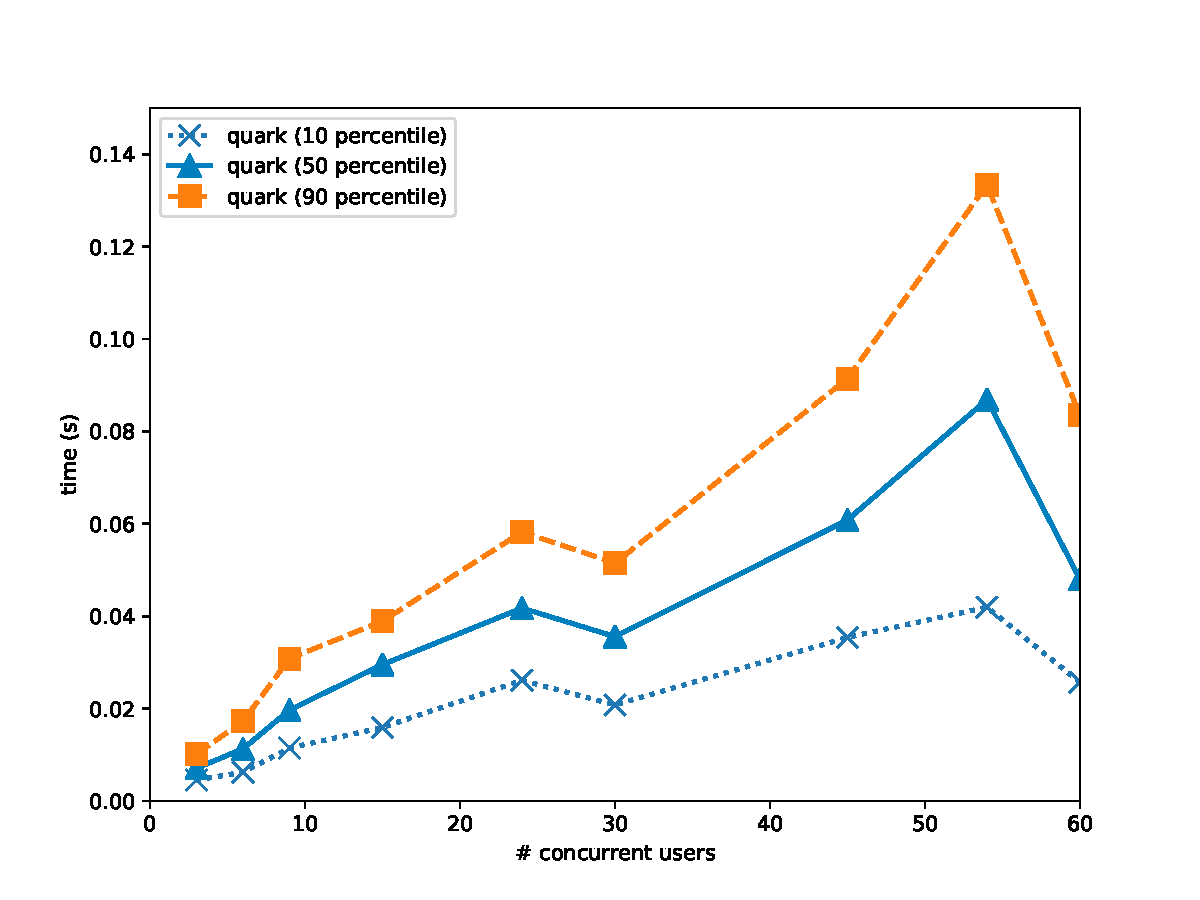
\includegraphics[scale=0.4]{Figures/rbmonkey_latency}
%   \caption{Latency of operations on a key-value store implemented
%   using a Red-Black tree MRDT.}
% \label{fig:rb-latency}
%   \vspace*{-0.2in}
% \end{figure}

\begin{figure}[ht]
  \centering
    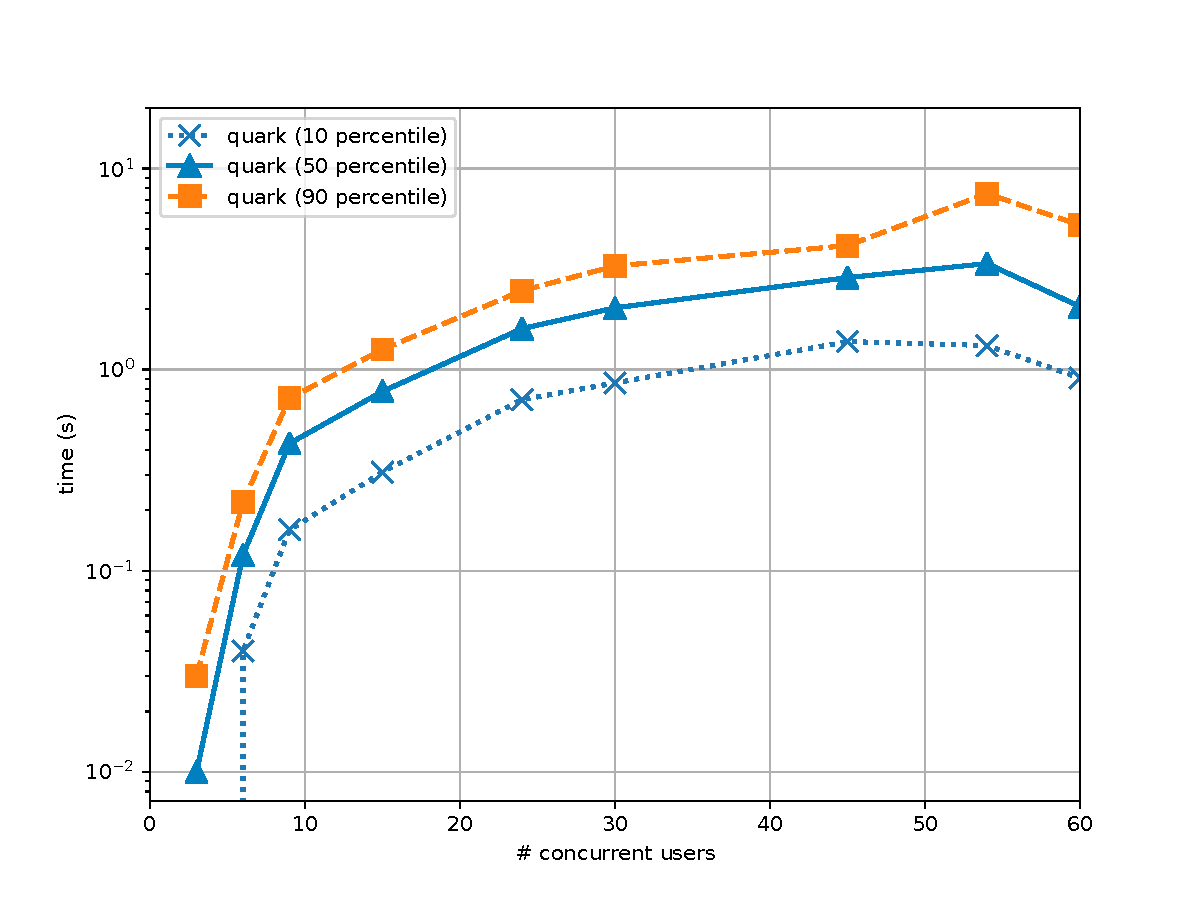
\includegraphics[scale=0.4]{Figures/rbmonkey_staleness}
  \caption{Staleness of key-value store merge operations.}
\label{fig:rb-staleness}
%\vspace*{-0.2in}
\end{figure}

We use the same experimental setup as before -- an increasing number
of concurrent processes perform a random operation on the local
version of the tree while merging with the remote versions in the
background.  Each process forks off a branch with an initial version
of an \C{RBTree} of size 1000, performs an insertion, updatation, or
deletion with probabilities of 0.5, 0.25, and 0.25. A new version of
the tree is committed after each operation. Each process performs 1000
operations with an inter-operation delay of 100ms. We measure the
latency of each tree operation and the staleness of each merge.
Latency measurements follow the same pattern as those for
collaborative editing (Fig.~\ref{fig:latency}), and have been elided.
The median latency remains around 50ms for most of the experiment.
Staleness measurements are plotted in Fig.~\ref{fig:rb-staleness}. As
before, staleness increases steadily in proportion to the increasing
number of concurrent processes. The 90th percentile staleness exceeds
1s for 15 concurrent processes, and 7s for 54 concurrent processes.
Unlike the collaborative applications, however, the number of replicas
in a conventional web application tends to be low, which could limit
staleness to a tolerable range. For instance, in the e-Commerce
application described above, 3 replicas of the shopping cart can be
kept in sync with each other with a 90th percentile lag (staleness) of
30ms.

Our experiments bring to the fore an inherent tradeoff among the
competing concerns of Convergent RDTs, namely (\rom{1}). The ease of
programming, (\rom{2}) Latency, and (\rom{3}).  Staleness. While CRDTs
try to optimize for latency and staleness, they require a significant
amount of development and verification effort to be expended to ensure
convergence. In contrast, \quark lets developers derive
convergent-by-construction MRDTs from ordinary data types that are
optimized for latency, but incur a non-trivial staleness overhead that
delays the time to convergence. 


